
\section{Présentation}
Le banc de test correspond au système composé du capteur \gls{capteur} et des appareils des mesures. Pour ce banc de test, le matériel suivant est utilisé :
\begin{itemize}
    \item \textbf{Capteur avec son support (Design 1 ou 5)}\\
          La géométrie générale du Design 1 et 5 est espliquée et représentée au chaptire \ref*{chap:catalogueSol}. \\

    \item \textbf{Débitmètre de référence FESTO SFAH-10B-Q6S-PNLK-PNVBA-M8}\\
          Le débitmètre choisi est un débitmètre bidirectionnel avec une entrée d'air de 6mm de diamètre. Il sera placé juste avant l'entrée du flux
          d'air dans le capteur, permettant ainsi d'avoir une valeur de référence fiable.\\

          Un graphe de la tension en fonction du débit fourni par le débitmètre de référence a été construit grâce à la sortie analogique de ce dernier :
          \begin{figure}[H]
              \centering
              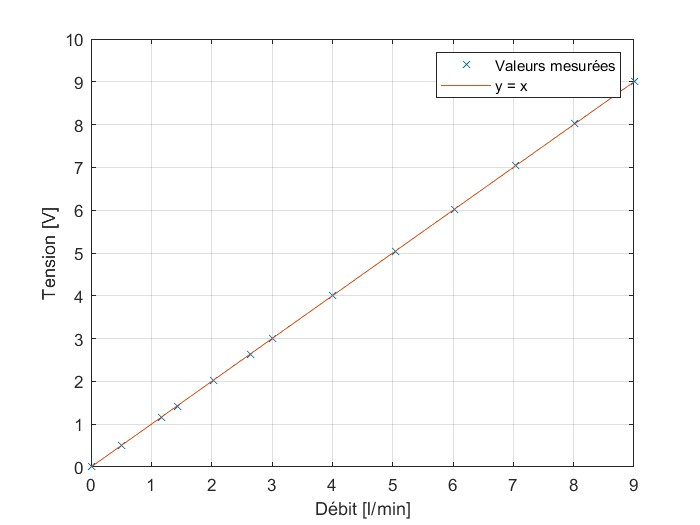
\includegraphics[scale = 0.4]{assets/figures/Calibration_maison.jpg}
              \caption{Tension en fonction du débit}
              \label{fig:calibration}
          \end{figure}

          Sur le figure \ref{fig:calibration}, nous pouvons observer la tension mesurée en fonction d'un certain débit d'air. Les paramètres utilisés
          pour cette calibration sont les suivants :
          \begin{itemize}
              \item Sortie analogique en tension sur une plage de 0V à 10V
              \item Full Scale allant de 0\% à +100\%
          \end{itemize}

          Le graphe montre une fonction linéaire qui se rapproche très fortement de la fonction $y = x$ (f$_{mesur\acute{e}}$(x) = 1.0004x - 0.0038).\\

    \item \textbf{Electrovanne FESTO MHE3-MS1H-3/2G-QS-6-K}\\
          Cette électrovanne fonctionne avec une tension de 24V.  Elle permet de créer un flux d'air pulsé. Ce flux d'air pulsé alimentera le
          capteur \gls{capteur}.\\
          Cet appareil possède 3 entrées/sorties disposées selon le schéma ci-dessous :
          \begin{figure}[H]
              \centering
              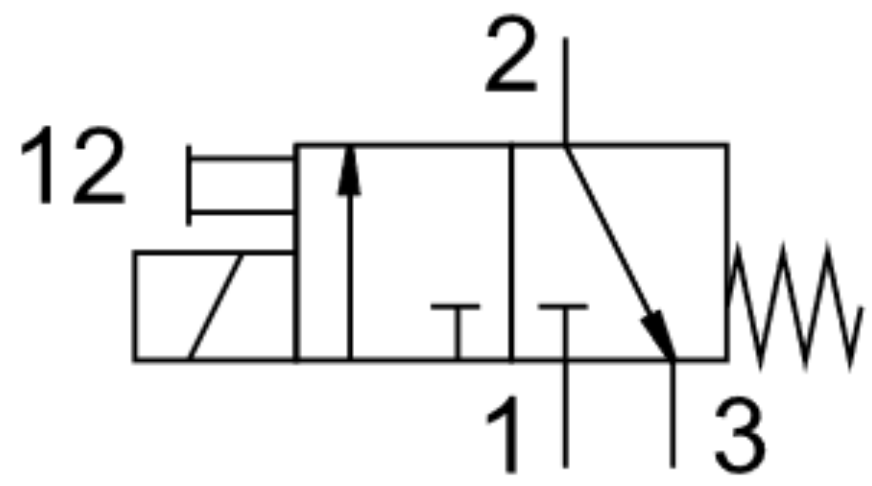
\includegraphics[scale = 0.3]{assets/figures/Electrovanne_InOutput.png}
              \caption{Entrée et sortie de l'électrovanne}
              \label{fig:electrovanne_InOutput}
          \end{figure}

    \item \textbf{Transistor MOSFET IRL540N}\\
          Le MOSFET (metal-oxide-semiconductor field-effect transistor) est un transistor fonctionnant en tension. Dans notre cas, il va
          être utilisé comme un interrupteur qui va alimenter ou non l'électrovanne.\\

    \item \textbf{Arduino Nano}\\
          L'Arduino Nano est un circuit-imprimé qui va également participer à la création du flux d'air pulsé. C'est grâce à l'arduino que la
          fréquence du flux d'air sera modulable. En effet, ce composant va contrôler le MOSFET, qui transmettra ensuite les informations à
          l'électrovanne.\\
          Le code utilisé afin de créer une sortie en tension par pulse est fourni en annexe.
\end{itemize}

Toutes les Datasheet des composants utilisés et achetés se trouvent en annexe. Ces Datasheet contiennent toutes les valeurs et schéma nécessaire
au dimensionnement du banc de test.

\section{Modélisation du banc de test}
\subsection{Flux d'air pulsé}
Une première solution est d'amener un flux d'air pulsé sur la membrane. Ce flux d'air serait contrôlé par une électrovanne et un
transistor MOSFET IRL540N. Ce transistor a été choisi car il permet d'être contrôlé grâce à un Arduino Nano. En effet, sa tension de seuil
($V_{GS}$) est de 4V, 5V ou 10V. Etant donné que l'Arduino Nano sortira une tension de 5V, cette valeur sera suffisante pour faire fonctionner
le MOSFET.
\begin{figure}[H]
    \centering
    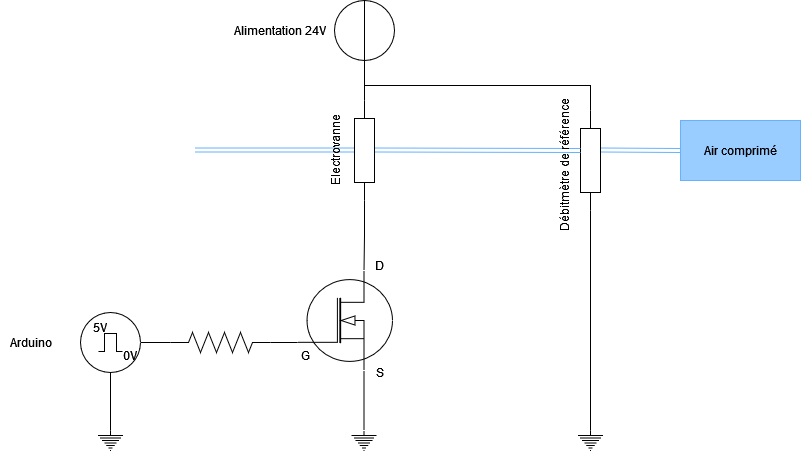
\includegraphics[scale=0.6]{assets/figures/MOSFET.png}
    \caption{Schéma électrique avec MOSFET}
    \label{fig:MOSFET}
\end{figure}
Un contrôle de la chaleur dégagée par effet Joule est utile afin de décider si un dissipateur thermique est nécessaire. Ce calcul se fait
de la manière suivante :\\
D'abord, calculons la chaleur dégagée (puissance par effet Joule) :

\[I_{electrovanne} = \frac{P_{electrovanne}}{U} = \frac{6.5}{24} \cong 0.27 A \]
\[P_{effetJoule} = R_{DS}\cdot I^2\]
Avec :\\
$R_{DS}$ (résistance entre les jonctions D et S du MOSFET) = 0.053

\begin{equation}
    P_{effetJoule} = 0.053\cdot 0.27^2 \cong 3.86mW
\end{equation}

Les différentes valeurs de résistances, puissances, etc. se trouvent dans la datasheet du MOSFET qui se trouve en annexe. \\

Puis, nous pouvons calculer la puissance maximum dissipée par le MOSFET :
\[P_{max\,dissip\acute{e}e} = \frac{max(T_j) - T_A}{R_{\theta JA}} = \frac{175-25}{62}\cong 2.42 W\]
Avec :\\
$T_j$ = température de jonction\\
$T_A$ = température ambiante\\
$R_{\theta JA}$ = résistance thermique, de jonction à ambiant

Ainsi, comme $P_{effetJoule} < P_{max\,dissip\acute{e}e}$, un dissipateur thermique n'est pas nécessaire. \\

Au niveau du fonctionnement général du système, le transistor est commandé par un Arduino Nano qui alimente le MOSFET avec 5V par pulsation (1 seconde à 5V et 1 seconde à 0V). \\
Lorsque le MOSFET reçoit 5V, il s'active et "laisse passer" le courant qui permet à l'électrovanne de s'ouvrir et de faire passer le
flux d'air.
\begin{figure}[H]
    \centering
    \begin{subfigure}[b]{0.45\textwidth}
        \hspace{-1.5cm}
        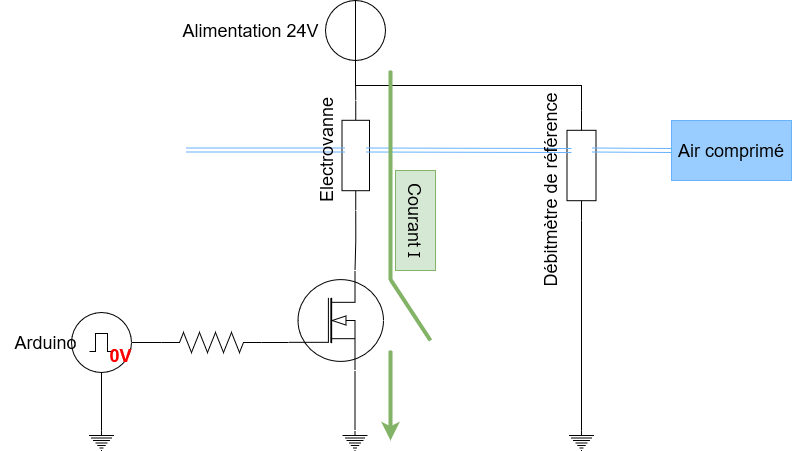
\includegraphics[scale = 0.3]{assets/figures/MOSFET_0V.png}
        \caption{MOSFET non-alimenté}
        \label{fig:MOSFET_0V}
    \end{subfigure}
    \begin{subfigure}[b]{0.45\textwidth}
        \centering
        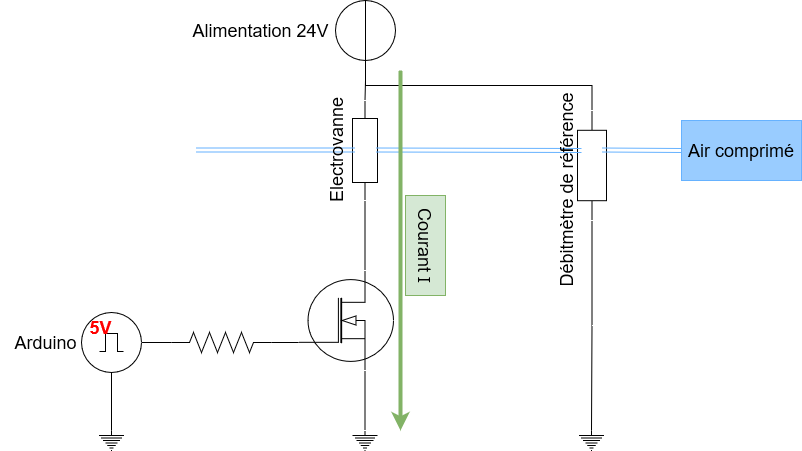
\includegraphics[scale = 0.3]{assets/figures/MOSFET_5V.png}
        \caption{MOSFET alimenté}
        \label{fig:MOSFET_5V}
    \end{subfigure}
    \caption{Fonctionnement du flux d'air pulsé}
    \label{fig:flux_pulse}
\end{figure}

Le corps de chauffe, constitué d'une fine couche d'or, doit être alimenté avec un certain courant. Ce courant, s'il est trop élevé, va abîmer la
membrane mais s'il est trop bas, il sera insuffisant pour entraîner une différence de température de part et d'autres du capteur. \\

Le calcul suivant a don été effectué afin de déterminer le courant à utiliser pour le corps de chauffe :
\[P_{max} = R\cdot I^2\]
Avec :\\
$P_{parSurface}$ (puissance max par unité de surface) = 100 $\frac{W}{m^2}$\\
$R$ (résistance du corps de chauffe) = 45 $\Omega$\\

La valeur de puissance par unité de surface a été tirée de la puissance maximale utilisée pour les chauffages du marché (chauffage au sol).
Elle permet d'avoir un ordre de grandeur pour la valeur de courant à fournir au corps de chauffe.
La surface du corps de chauffe à été approximée à 80 mm$^2$ ($2mm x 40mm$).\\
Ainsi une règle de 3 a été effectuée afin de trouver la valeur de puissance pour le corps de chauffe concerné :
\[P_{max} = 8\cdot 10^{-5}\cdot 100 = 1.78\cdot 10^{-4}\]
\[I = \sqrt{\frac{P_{max}}{R}} = \sqrt{\frac{1.78\cdot 10^{-4}}{45}} \cong 13 mA\]
Plusieurs tests ont été alors effectué dans une plage de 10 mA à 20 mA. Ces tests ont donné un courant maximum a 15 mA. Au-delà, la membrane
est abîmée (couche d'or rongée).\\

\subsection{Conception 3D}
\begin{figure}[H]
    \centering
    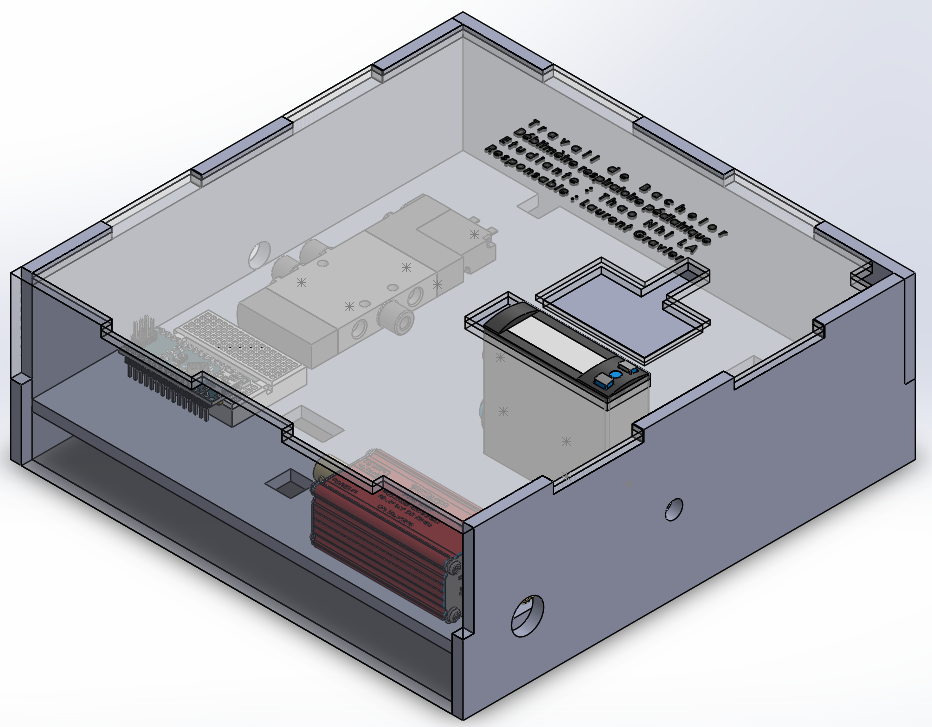
\includegraphics[scale = 0.5]{assets/figures/Banc_de_test.png}
    \caption{Conception 3D du banc de test}
    \label{fig:3D_banc_test}
\end{figure}

\subsection{Corps de chauffe pulsé}

\section{Vérification du banc de test}
La première version du banc de test est pratique, car lors de la mise en pratique, le flux d'air pulsé est aisément vérifiable. \\
Cependant, lors des premiers tests, aucun signal n'était visible sur l'oscilloscope. Ceci peut être dû à différentes raisons :
\begin{itemize}
    \item Un mauvais contact avec les pointes ressorts\\

    \item La puissance du corps de chauffe n'est pas suffisante\\

    \item L'échantillon (capteur \gls{capteur}) est défectueux\\
\end{itemize}

Afin de vérifier quel-s paramètre-s entraîne-nt un mauvais résultat, une première décision a été de tester le \gls{capteur} ouvert (sans son support,
en utilisant seulement la membrane).
Des pinces plates viennent faire le contact électrique directement sur les couches d'or afin de mesurer la tension y circulant.
\begin{figure}[H]
    \centering
    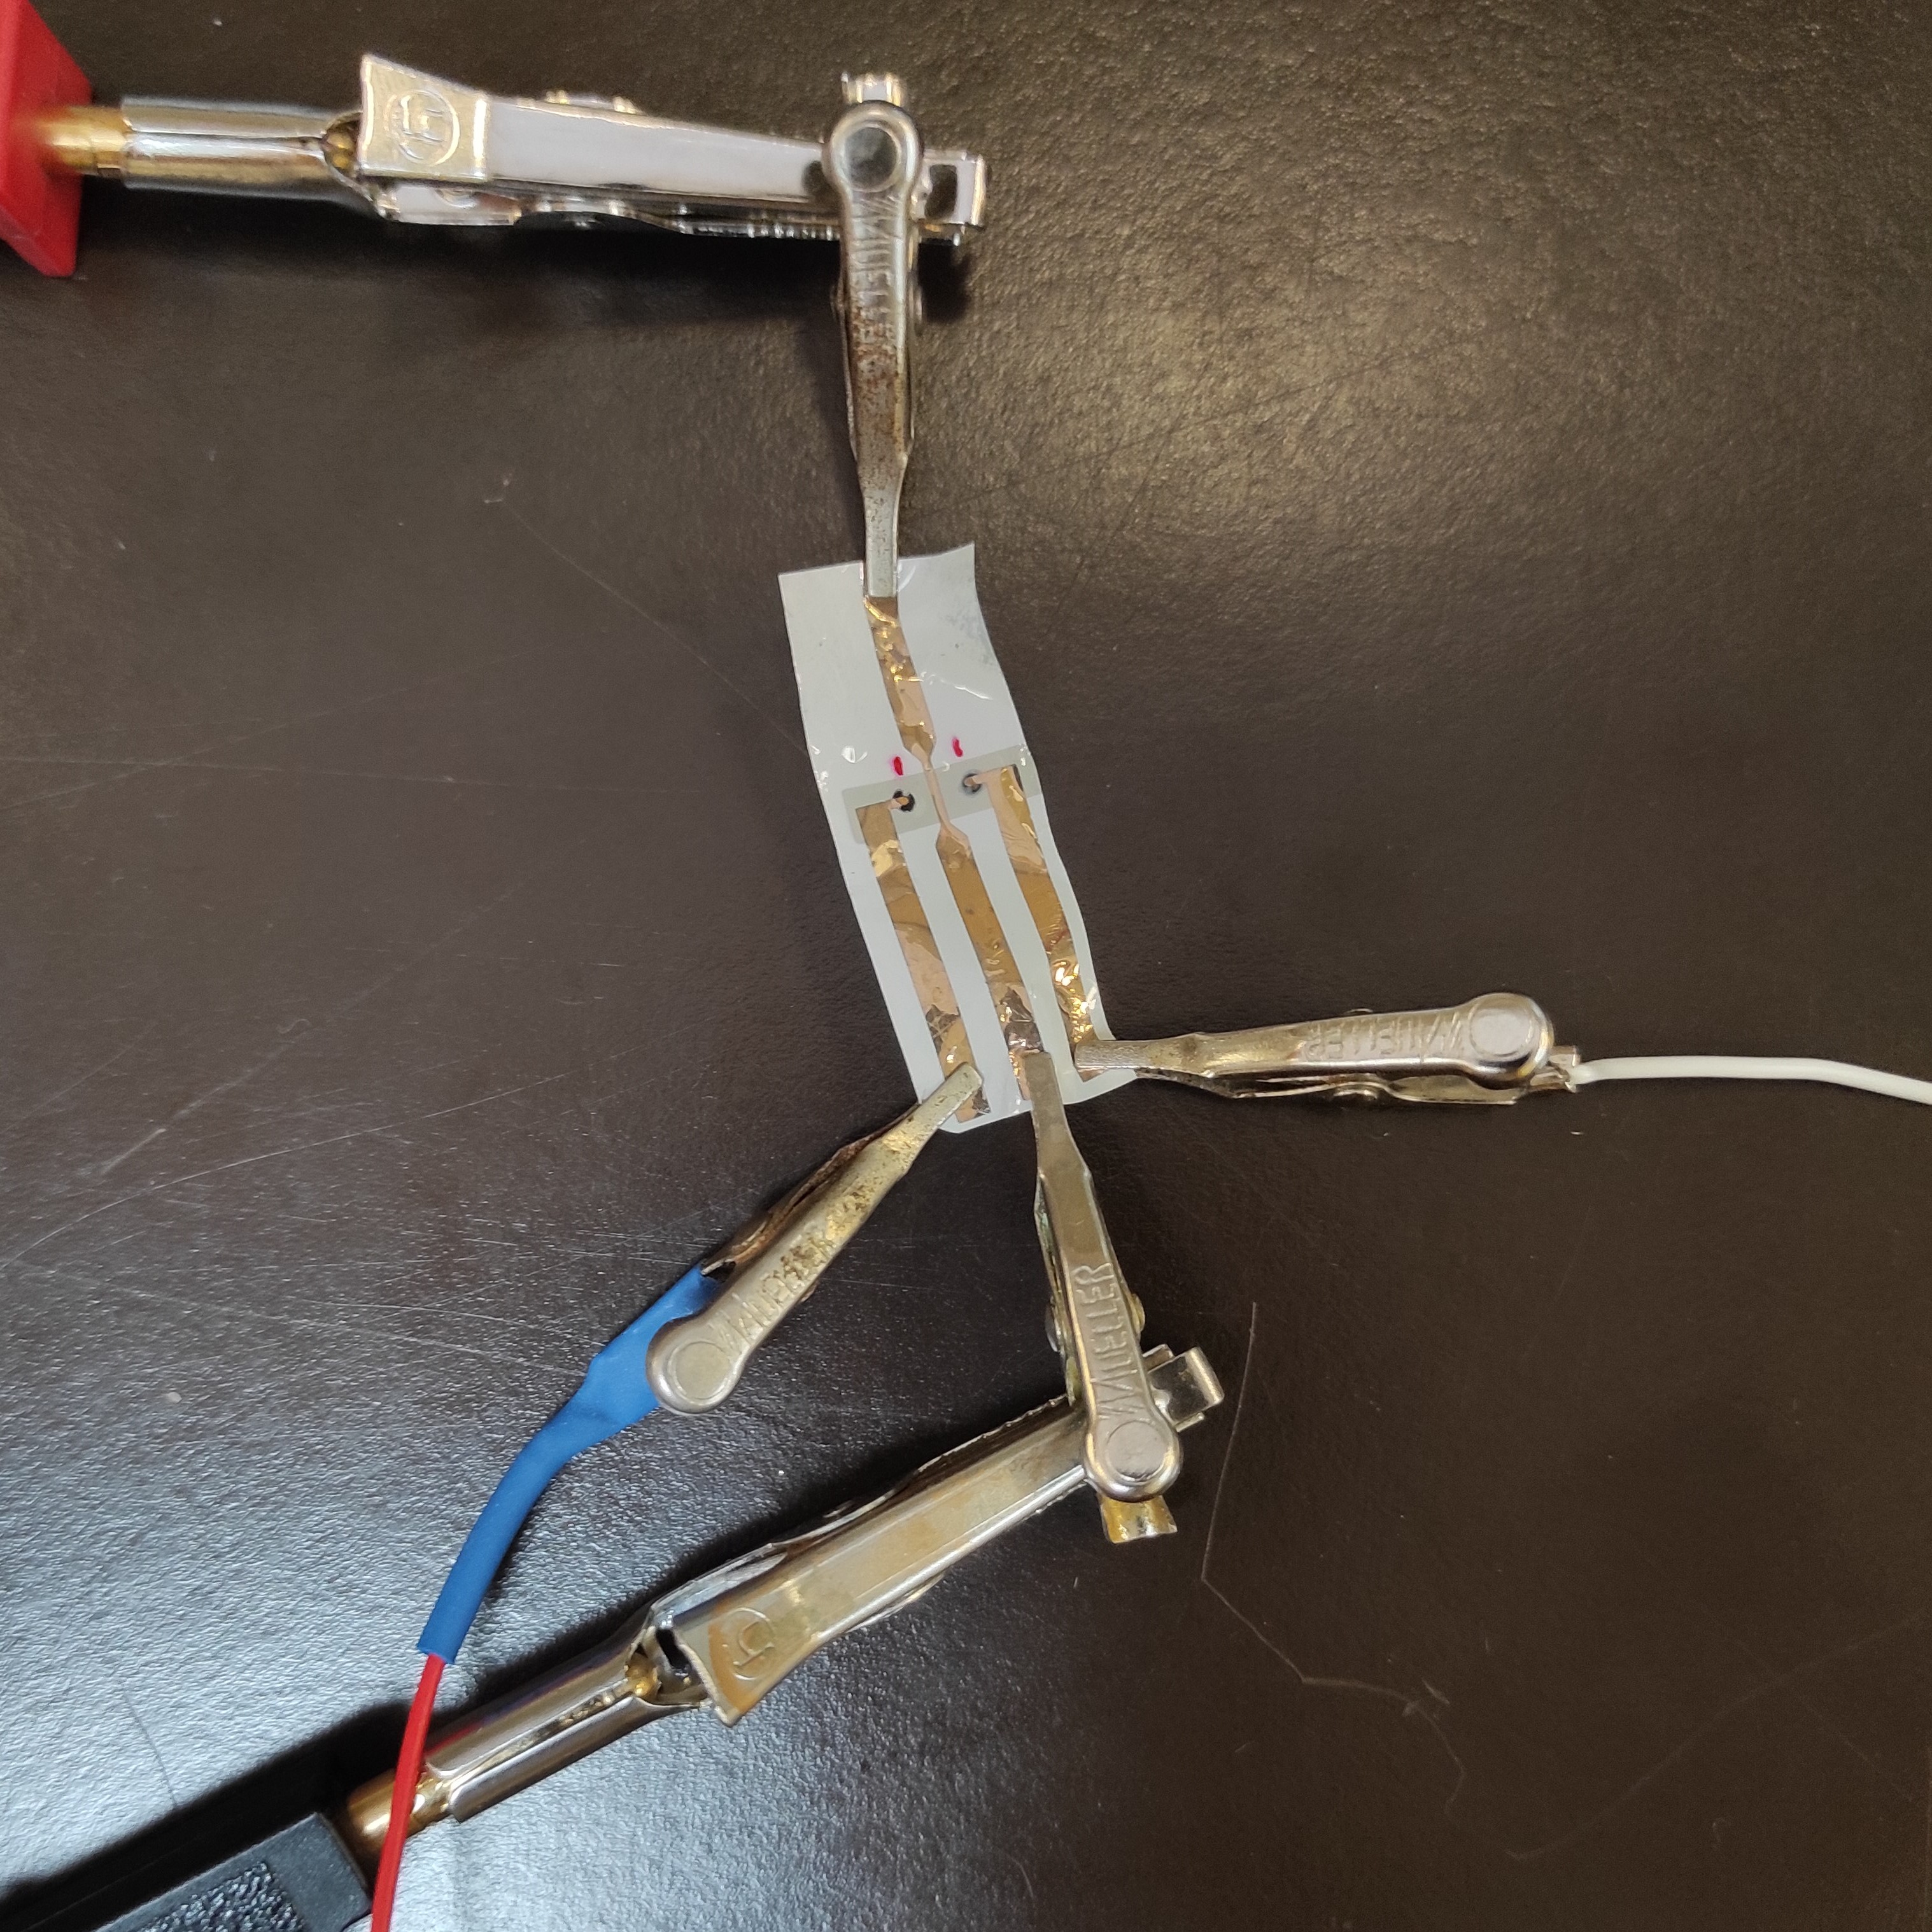
\includegraphics[scale = 0.05]{assets/figures/CapteurOuvert.jpg}
    \caption{Tests sur capteur ouvert}
    \label{fig:capteurOuvert}
\end{figure}
Cette installation ne communiquait pas non plus de résultat concluant (tension à 0V). \\

Le corps de chauffe a donc été mis en question. Une alternative à ce corps de chauffe a été de venir toucher la pince plate d'un côté du
capteur afin d'engendrer une différence de température entre les deux parties coudées. Ceci a bel et bien entraîné une différence de
température et donc, une tension. Cependant, cette dernière provient de la différence de température entre l'or (sur la membrane) et le métal
de la pince plate. \\

Afin de chauffer une des deux parties électrodéposées, une court tube a été utilisé. Un flux d'air chaud a été soufflé directement sur cette
partie afin de créer un gradient de température mais à nouveau, auncune fluctuation n'a été perçue. Cependant, lorsque le flux d'air chaud
était soufflé au niveau de la pince plate, une plus grande fluctuation de tension était visible. Cela signifie que la jonction avec le tellure
de bismuth est probablement pathologique.\\

Il était tout de même nécessaire et intéressant de vérifier si le banc de test fonctionnait de manière appropriée. Pour cela, un autre capteur
a été utilisé afin de vérifier la fonctionalité du banc de test. \\
Le capteur utilisé est un capteur infrarouge par nanotechnologie qui traduit un certain rayonnement électromagnétique en tension. Ainsi lorsque l'on souffle
dessus, un changement dans l'environnement, et plus précisément dans la température ambiante, aura lieu. Ce flux d'air impacte donc
les rayonnements thermiques qui, eux, sont étroitement liés, entre autres, aux rayonnements infrarouges. C'est donc pour cette raison qu'à
l'oscilloscope, une fluctuation sur la tension se dessine.
\begin{figure}[H]
    \centering
    \begin{subfigure}[b]{0.45\textwidth}
        \hspace{-1 cm}
        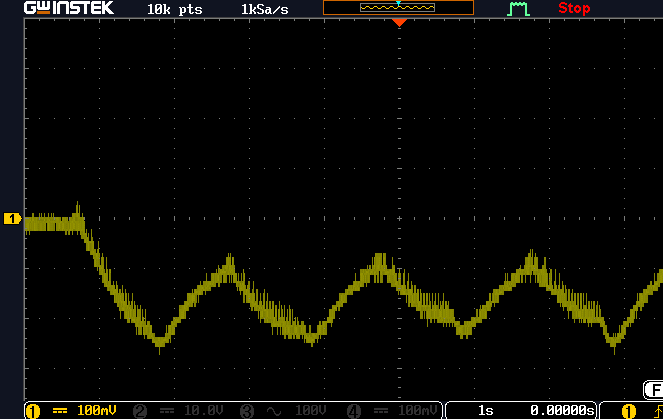
\includegraphics[scale = 0.45]{assets/figures/CapteurIR_1s_1s.PNG}
        \caption{Air pulsé pendant 1s puis repos pendant 1s}
        \label{fig:1s1s}
    \end{subfigure}
    \begin{subfigure}[b]{0.45\textwidth}
        \centering
        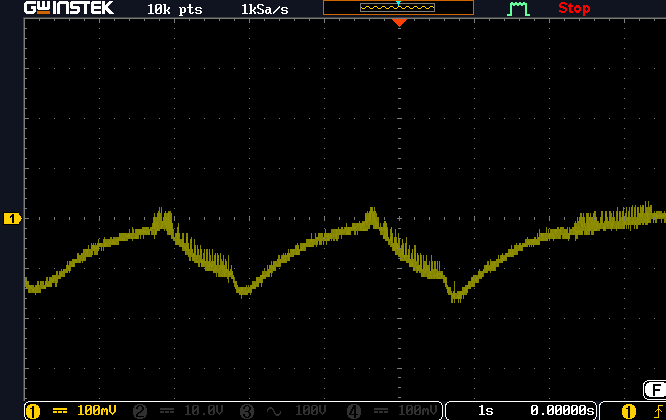
\includegraphics[scale = 0.45]{assets/figures/1_8s_repos.PNG}
        \caption{Air pulsé pendant 1s puis repos pendant 1.8s}
        \label{fig:1_8s}
    \end{subfigure}
    \caption{Résultats avec capteur infrarouge}
    \label{fig:capteurIR}
\end{figure}

Les figures ci-dessus (\ref{fig:capteurIR}), montrent que le banc de test et plus précisément, le système de flux d'air pulsé accompagné de
la sortie à l'oscilloscope (en passant par l'amplificateur) fonctionne bien. En effet, sur les figures \ref*{fig:1s1s} et \ref*{fig:1_8s}
les différentes pulsations sont bien visibles.\\

Sur la figure \ref*{fig:1s1s}, la récupération du capteur est plus longue que le temps de repos. C'est pourquoi le temps de repos a été allongé
et fixé à 1.8s (figure \ref*{fig:1_8s}). Ceci permet au capteur de se remettre à zéro et permet aussi de contrôler que la fréquence est bien
modulable. \\

Une autre partie intéressante à étudier est l'amplificateur. Pour ce faire, un petit programme LabView a été utilisé afin de mesurer, dans un
premier temps, la réponse du capteur \gls{infrarouge} sans amplificateur, puis, dans un second temps, la réponse avec amplificateur. Ceci nous
permettra de qualifier l'amplificateur.

Ces tests prouvent que le banc de test semble fonctionner de manière correcte. L'échantillon est alors certainement le facteur engendrant de
mauvais résultats. Un développement de cette thématique sera effectué dans le chapitre \ref{chap:mesures}.

\subsection{Procédure d'utilisation du banc de test}
